\section{Graph Algorithms}

	\begin{frame}
          \frametitle{Graphs}

          Pervasive data structure in Computer Science---an abstract
          representation in use to describe different domains, including
          trasport systems, electrical circuits, human interactions (social networks),
          computer networks, and software dependencies. \pause This class aims to
          discuss two concerns:   

          \vskip+1.5em

          \begin{itemize}
            \item graph representation 
            \item graph algorithms 
          \end{itemize}
        \end{frame}

\begin{frame}
\frametitle{Definition}

A graph $G$ is a pair $(V, E)$ where $V$ is an arbitrary
set and $E$ is a subset of $V^{(2)}$\pause---the set of all pairs of
elements in $V$.  The elements of $V$ are the {\color{blue}vertices} of the
graph, while the elements of $E$ are the {\color{blue}edges}
of the graph. 


\pause \vskip+1.5em
\begin{block}{Different flavors of graphs}

\begin{itemize}
\item directed graphs $\times$ undirected graphs
\item weighted graphs $\times$ unweighted graphs
\item ciclic graphs $\times$ aciclic graphs
\item \ldots
\end{itemize}
\end{block}
\end{frame}

\begin{frame}
\frametitle{Graph representations}


\begin{itemize}
\item {\bf Adjacency-list:} compact representation recommended for
  {\color{blue}sparse graphs}  (where $|E|$ is smaller than 
  $|V|^{2}$). \pause 

\item {\bf Adjacency-matrix:} recommended for dense graphs or when we
  need to frequently search if an edge $(v_1, v_2)$ exists.   
\end{itemize}

\end{frame}

\begin{frame}
\frametitle{Samples (Fonte: Introduction to Algorithms)}
\centering{

\includegraphics[scale=0.5]{images/undirected01.png}

\pause 

\includegraphics[scale=0.5]{images/directed01.png}	
}

\end{frame}


\begin{frame}
  \frametitle{Graph Algorithms}

  \begin{itemize}
   \item Search: Breadth-first search and Depth-first Search
   \item Single-source shortest paths: Bellman-Ford and Dijkstra algorithms
   \item {\color{blue}All-pairs shortest paths}  
   \item {\color{blue}Minimum Spanning Trees}
  \end{itemize}
\end{frame}


\begin{frame}{All-pairs shortest paths}

  We are given a weighted, directed graph $G(V, E)$ with a
  weight function $w : E \rightarrow \mathbb{R}$, and our goal
  is to find, for {\color{blue}every} pair of vertices $u, v \in V$,
  the shortest path from $u$ to $v$.

  \pause

  \begin{block}{Note}
  \begin{itemize}
    \item Computing the single-source shortest paths to all
      vertices $v \in V$ is not efficient. \pause Here we will present a
      dynamic programming algorithm (Floyd-Warshal) that runs in $\Theta(V^3)$ 
  \end{itemize}
  \end{block}

\end{frame}

\begin{frame}{Floyd-Warshal algorithm}

  \begin{block}{Features}
    \begin{itemize}
     \item Represents the graph using an adjacency-matrix \pause (each cell $(u, v)$ in
       the matrx contains the weight of the edge $u \rightarrow v$). \pause

     \item Considers the intermediate vertices of a shortest path. If $p = \rangle v_1, v_2, \ldots, v_l \langle$,
       any vertex other than $v_1$ and $v_l$ are intermediate vertices. \pause

     \item Iterative: Under the assumption that $V = \{1, 2, \ldots, n\}$, considers the subsets $\{1, 2, \ldots, k\}$
       of vertices for some $k$. 
    \end{itemize}
  \end{block}
\end{frame}

\begin{frame}
  \centering{
    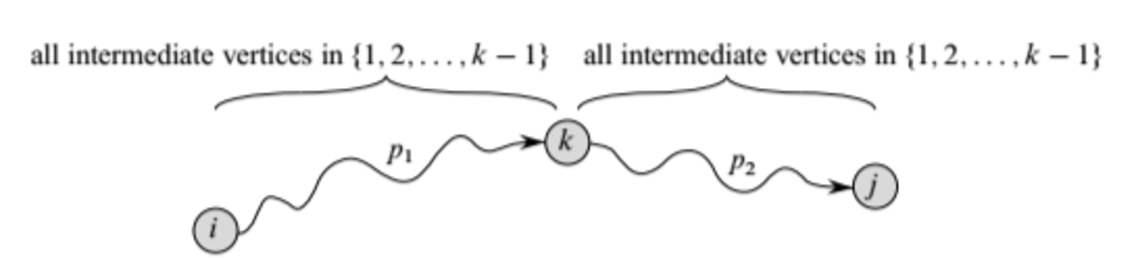
\includegraphics[scale=0.5]{images/fw}
   }
\end{frame}

\begin{frame}{Recursive Solution}

\[
d^{(k)}_{ij}= \left\{
\begin{array}{ll}
      w_{ij}                    & if\ k = 0\\ 
      min(d^{(k-1)}_{ij}, d^{(k-1)}_{ik}+d^{(k-1)}_{kj})  & if\ k \geq 1 \\   
\end{array} 
\right. 
\]

\pause

\begin{itemize}
  \item The matrix $D^{(n)}$ gives the final answer (considering $V = \{1, 2, \ldots, n\}$).
\end{itemize}
\end{frame}

\begin{frame}{Example}
    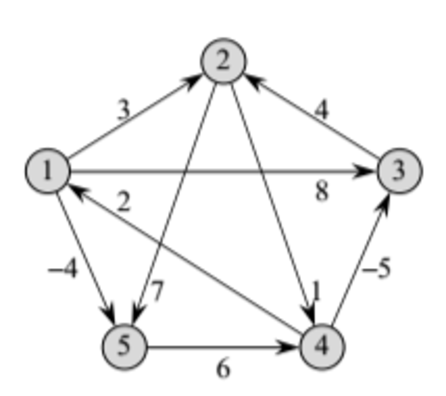
\includegraphics[scale=0.5]{images/graph-fw}
\end{frame}

\begin{frame}
  \centering{
    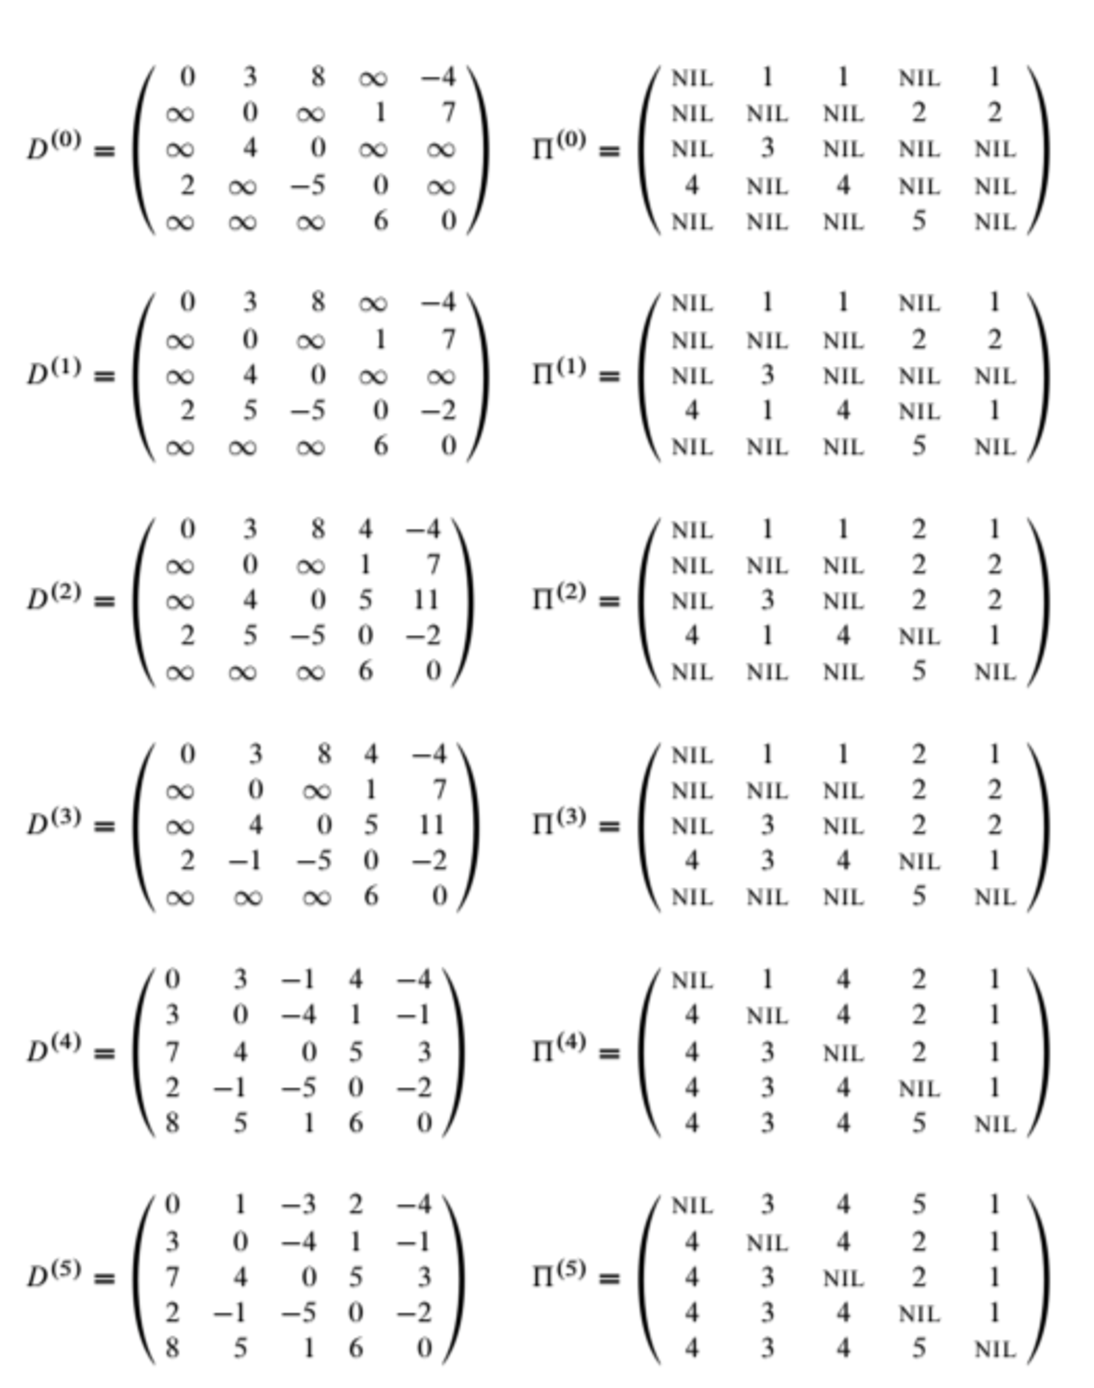
\includegraphics[scale=0.3]{images/fw-res}}
\end{frame}

\begin{frame}
  \begin{block}{Floyd-Warshall algorithm}
      \begin{algorithmic}
    \Procedure{Floyd-Warshall}{W}
     \State $n = W.rows$
     \State $D^{(0)} = W$
     \For{$k = 1 \ldots n$}
      \State $D^{(k)} = (d^{(k)}_{ij}) \text{ be a new n x n matrix}$
      \For{$i = 1 \ldots n$}
        \For{$j = 1 \ldots n$}
          \State $d^{(k)}_{ij} = min(d^{(k-1)}_{ij}, d^{(k-1)}_{ik}+d^{(k-1)}_{kj})$
        \EndFor
      \EndFor
     \EndFor
    \State {\bf return} $D^{(n)}$
    \EndProcedure 
  \end{algorithmic}
  \end{block}  
\end{frame}

\begin{frame}{Minimum Spanning Trees}

  Given a connected, weighted, and undirected graph $G = (V, E)$, we wish to
  find an acyclic subset $T \subseteq E$ that connects all of the vertices
  and whose {\color{blue}total} weight is minimized. \pause Since $T$ is acyclic and
  connects all of the vertices, it must form a (spanning) tree. 

  \pause \vskip+1.5em

  \centering{
    \includegraphics[scale=0.5]{images/st}
  }
\end{frame}


\begin{frame}

  The book presents an interesting description of the algortihms for
  Minimum Spanning Trees: a generic method for growing minimum spanning trees
  and two implementations of the algorithm (Kruskal's algorithm and Prim's algorithm).

  \pause \vskip+1.5em

  \begin{block}{Generic Method}
  \begin{algorithmic}
    \Procedure{Generic-MST}{G, w}
     \State $A = \emptyset$                 
     \While{$\text{A does not form a spanning tree}$}        
       \State $\text{find an edge (u, v) that is safe for A}$
       \State $A = A \cup \{(u, v)\}$
     \EndWhile
     \State {\bf return} $A$
    \EndProcedure
  \end{algorithmic}
  \end{block}

  \pause

  \begin{itemize}
    \item The challenge is to find out a {\color{blue}safe edge (u, v)}. 
  \end{itemize}
\end{frame}

\begin{frame}{Definitions}

  \begin{itemize}
   \item A {\color{blue}$cut(S, V-S)$} of an undirected graph $G = (V, E)$ is a partition of $V$. \pause 

   \item An {\color{blue}edge $(u, v) \in E$ crosses} a $cut(S, V-S)$ if one of its endpoints is in $S$ and
     the other is in $V-S$. \pause

   \item A {\color{blue}cut respects} a set A of edges if no edge in A crosses the cut. \pause
     
   \item An edge is a {\color{blue}light edge crossing} a cut if its weight is the minimum of any
     edge crossing the cut.  
  \end{itemize}
\end{frame}

\begin{frame}
  \begin{block}{Theorem}
    Given:
    \begin{itemize}
      \item $G = (V, E)$ is a connected, undirected graph
      \item $w : E \rightarrow \mathbb{R}$ is a weighted function.
      \item $A$ is a subset of $E$ (included in some minimum spanning subtree for $G$)
      \item $(S, V-S)$ is any cut of $G$ that respects $A$
      \item $(u, v)$ is a light edge crossing $(S, V-S)$
    \end{itemize}
    then, edge $(u, v)$ is safe for $A$. 
  \end{block}

  Both algorithm implementations relie on this theorem. 
\end{frame}

\begin{frame}
  In the Kruskal's algorithm, the set $A$ is a {\color{blue}forest}
  whose vertices are all those of the given graph. The safe edge
  added to $A$ is allways a lest-weight edge in the graph that
  connects two distinct trees in the forest. \pause The book
  shows an implementation that benefits from the Disjoint Set
  data structure, whose interface contains three operations:
  \texttt{makeSet}, \texttt{findSet}, and \texttt{union}. 
\end{frame}

\begin{frame}
  \begin{small}
  \begin{algorithmic}
    \Procedure{MST-Kruskal}{G, w}
    \For{$\text{each vertex v } \in G.V$}
      \State $makeSet(v)$
    \EndFor
    \State $lst = \text{sort the edges of G.E into nondecreasing order by weight w}$
    \For{$(u, v) \rightarrow lst$}
      \If{$findSet(u) \neq findSet(v)$}
       \State $A = A \cup \{(u, v)\}$
       \State $union(u, v)$
      \EndIf 
    \EndFor
    \State {\bf return} $A$  
    \EndProcedure
  \end{algorithmic}
  \end{small}
\end{frame}

\begin{frame}{TODO}

  Study and implement the Prim's algorithm for
  computing minimum spanning trees. 
 
\end{frame}
